\documentclass[si.tex]{subfiles}
\begin{document}

For the orientation perception data, we show fits at one level or at five levels of noise at 1K trials in Figure~\ref{fig:gardelle-one-level-pri-enc}.

For the time interval perception data, we show model fit statistics when either presupposing a Weber's law-based encoding (as in the main paper) or a freely fitted encoding (alternative) in Figure~\ref{fig:remington-nll-free-or-weber}; even in the latter case, data generated from a bimodal prior enables identifiability.



\begin{comment}

for i in 0; do
python3 RunGardelle_FreePrior_ZeroTrig_Downsampled_TargetSize_VIZ_EncPri.py $i 0 10.0 180 1-2-3-4-5 1000 21
python3 RunGardelle_FreePrior_ZeroTrig_Downsampled_TargetSize_VIZ_EncPri.py $i 0 10.0 180 1 1000 21
python3 RunGardelle_FreePrior_ZeroTrig_Downsampled_TargetSize_VIZ_EncPri.py $i 0 10.0 180 2 1000 21
python3 RunGardelle_FreePrior_ZeroTrig_Downsampled_TargetSize_VIZ_EncPri.py $i 0 10.0 180 3 1000 21
python3 RunGardelle_FreePrior_ZeroTrig_Downsampled_TargetSize_VIZ_EncPri.py $i 0 10.0 180 4 1000 21
python3 RunGardelle_FreePrior_ZeroTrig_Downsampled_TargetSize_VIZ_EncPri.py $i 0 10.0 180 5 1000 21
python3 RunGardelle_FreePrior_ZeroTrig_Downsampled_TargetSize_VIZ_EncPri.py $i 0 10.0 180 1 2000 21
python3 RunGardelle_FreePrior_ZeroTrig_Downsampled_TargetSize_VIZ_EncPri.py $i 0 10.0 180 2 2000 21
python3 RunGardelle_FreePrior_ZeroTrig_Downsampled_TargetSize_VIZ_EncPri.py $i 0 10.0 180 3 2000 21
python3 RunGardelle_FreePrior_ZeroTrig_Downsampled_TargetSize_VIZ_EncPri.py $i 0 10.0 180 4 2000 21
python3 RunGardelle_FreePrior_ZeroTrig_Downsampled_TargetSize_VIZ_EncPri.py $i 0 10.0 180 5 2000 21
done

for i in 1; do
python3 RunGardelle_FreePrior_L1Loss_Downsampled_TargetSize_VIZ_EncPri.py $i 0 10.0 180 1-2-3-4-5 1000 21
python3 RunGardelle_FreePrior_L1Loss_Downsampled_TargetSize_VIZ_EncPri.py $i 0 10.0 180 1 1000 21
python3 RunGardelle_FreePrior_L1Loss_Downsampled_TargetSize_VIZ_EncPri.py $i 0 10.0 180 2 1000 21
python3 RunGardelle_FreePrior_L1Loss_Downsampled_TargetSize_VIZ_EncPri.py $i 0 10.0 180 3 1000 21
python3 RunGardelle_FreePrior_L1Loss_Downsampled_TargetSize_VIZ_EncPri.py $i 0 10.0 180 4 1000 21
python3 RunGardelle_FreePrior_L1Loss_Downsampled_TargetSize_VIZ_EncPri.py $i 0 10.0 180 5 1000 21
python3 RunGardelle_FreePrior_L1Loss_Downsampled_TargetSize_VIZ_EncPri.py $i 0 10.0 180 1 2000 21
python3 RunGardelle_FreePrior_L1Loss_Downsampled_TargetSize_VIZ_EncPri.py $i 0 10.0 180 2 2000 21
python3 RunGardelle_FreePrior_L1Loss_Downsampled_TargetSize_VIZ_EncPri.py $i 0 10.0 180 3 2000 21
python3 RunGardelle_FreePrior_L1Loss_Downsampled_TargetSize_VIZ_EncPri.py $i 0 10.0 180 4 2000 21
python3 RunGardelle_FreePrior_L1Loss_Downsampled_TargetSize_VIZ_EncPri.py $i 0 10.0 180 5 2000 21
done

for i in 2 4 6 8; do
python3 RunGardelle_FreePrior_CosineLoss_Downsampled_TargetSize_VIZ_EncPri.py $i 0 10.0 180 1-2-3-4-5 1000 21
python3 RunGardelle_FreePrior_CosineLoss_Downsampled_TargetSize_VIZ_EncPri.py $i 0 10.0 180 1 1000 21
python3 RunGardelle_FreePrior_CosineLoss_Downsampled_TargetSize_VIZ_EncPri.py $i 0 10.0 180 2 1000 21
python3 RunGardelle_FreePrior_CosineLoss_Downsampled_TargetSize_VIZ_EncPri.py $i 0 10.0 180 3 1000 21
python3 RunGardelle_FreePrior_CosineLoss_Downsampled_TargetSize_VIZ_EncPri.py $i 0 10.0 180 4 1000 21
python3 RunGardelle_FreePrior_CosineLoss_Downsampled_TargetSize_VIZ_EncPri.py $i 0 10.0 180 5 1000 21
python3 RunGardelle_FreePrior_CosineLoss_Downsampled_TargetSize_VIZ_EncPri.py $i 0 10.0 180 1 2000 21
python3 RunGardelle_FreePrior_CosineLoss_Downsampled_TargetSize_VIZ_EncPri.py $i 0 10.0 180 2 2000 21
python3 RunGardelle_FreePrior_CosineLoss_Downsampled_TargetSize_VIZ_EncPri.py $i 0 10.0 180 3 2000 21
python3 RunGardelle_FreePrior_CosineLoss_Downsampled_TargetSize_VIZ_EncPri.py $i 0 10.0 180 4 2000 21
python3 RunGardelle_FreePrior_CosineLoss_Downsampled_TargetSize_VIZ_EncPri.py $i 0 10.0 180 5 2000 21
done
\end{comment}



\begin{figure}
\centering

Fitting at $p=0$

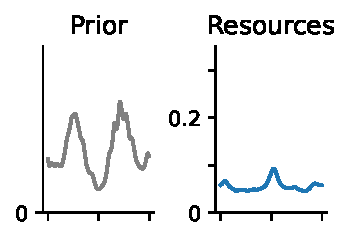
\includegraphics[width=0.15\textwidth]{figures/RunGardelle_FreePrior_ZeroTrig_Downsampled_TargetSize_VIZ_EncPri.py_0_0-21_10.0_180_1000_1.pdf}
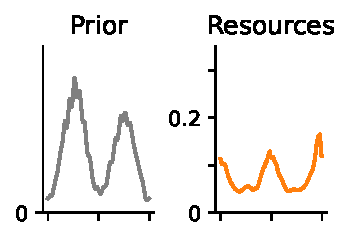
\includegraphics[width=0.15\textwidth]{figures/RunGardelle_FreePrior_ZeroTrig_Downsampled_TargetSize_VIZ_EncPri.py_0_0-21_10.0_180_1000_2.pdf}
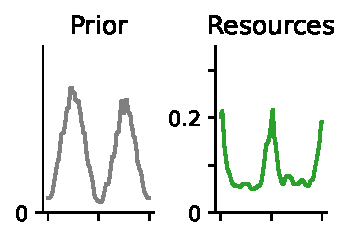
\includegraphics[width=0.15\textwidth]{figures/RunGardelle_FreePrior_ZeroTrig_Downsampled_TargetSize_VIZ_EncPri.py_0_0-21_10.0_180_1000_3.pdf}
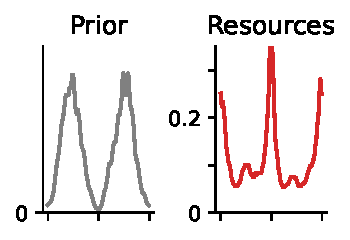
\includegraphics[width=0.15\textwidth]{figures/RunGardelle_FreePrior_ZeroTrig_Downsampled_TargetSize_VIZ_EncPri.py_0_0-21_10.0_180_1000_4.pdf}
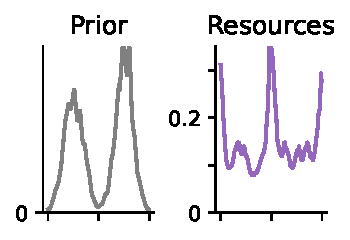
\includegraphics[width=0.15\textwidth]{figures/RunGardelle_FreePrior_ZeroTrig_Downsampled_TargetSize_VIZ_EncPri.py_0_0-21_10.0_180_1000_5.pdf}
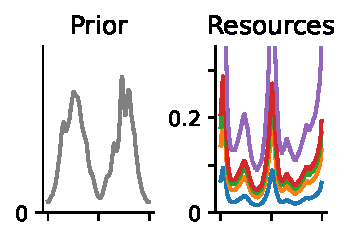
\includegraphics[width=0.15\textwidth]{figures/RunGardelle_FreePrior_ZeroTrig_Downsampled_TargetSize_VIZ_EncPri.py_0_0-21_10.0_180_1000_1-2-3-4-5.pdf}


Fitting at $p=1$

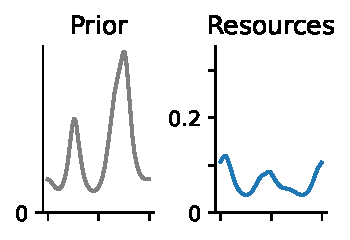
\includegraphics[width=0.15\textwidth]{figures/RunGardelle_FreePrior_L1Loss_Downsampled_TargetSize_VIZ_EncPri.py_1_0-21_10.0_180_1000_1.pdf}
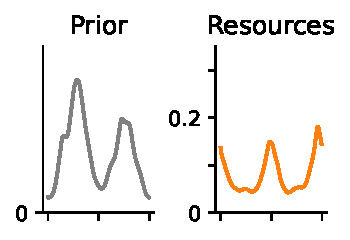
\includegraphics[width=0.15\textwidth]{figures/RunGardelle_FreePrior_L1Loss_Downsampled_TargetSize_VIZ_EncPri.py_1_0-21_10.0_180_1000_2.pdf}
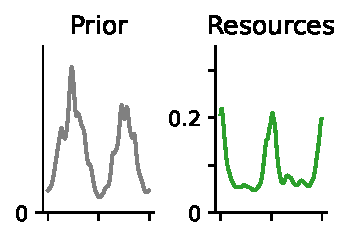
\includegraphics[width=0.15\textwidth]{figures/RunGardelle_FreePrior_L1Loss_Downsampled_TargetSize_VIZ_EncPri.py_1_0-21_10.0_180_1000_3.pdf}
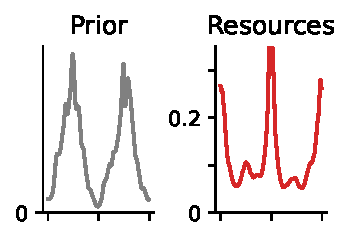
\includegraphics[width=0.15\textwidth]{figures/RunGardelle_FreePrior_L1Loss_Downsampled_TargetSize_VIZ_EncPri.py_1_0-21_10.0_180_1000_4.pdf}
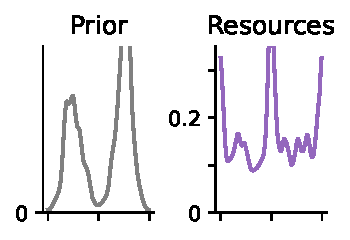
\includegraphics[width=0.15\textwidth]{figures/RunGardelle_FreePrior_L1Loss_Downsampled_TargetSize_VIZ_EncPri.py_1_0-21_10.0_180_1000_5.pdf}
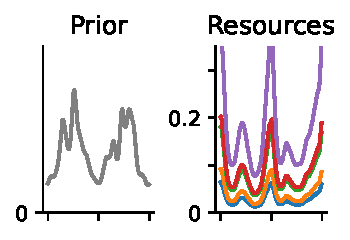
\includegraphics[width=0.15\textwidth]{figures/RunGardelle_FreePrior_L1Loss_Downsampled_TargetSize_VIZ_EncPri.py_1_0-21_10.0_180_1000_1-2-3-4-5.pdf}


Fitting at $p=2$

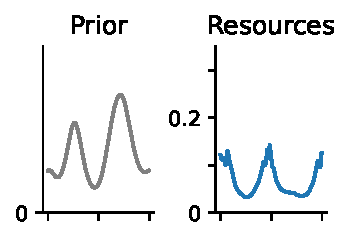
\includegraphics[width=0.15\textwidth]{figures/RunGardelle_FreePrior_CosineLoss_Downsampled_TargetSize_VIZ_EncPri.py_2_0-21_10.0_180_1000_1.pdf}
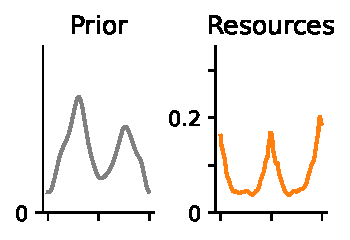
\includegraphics[width=0.15\textwidth]{figures/RunGardelle_FreePrior_CosineLoss_Downsampled_TargetSize_VIZ_EncPri.py_2_0-21_10.0_180_1000_2.pdf}
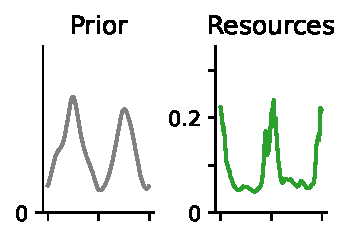
\includegraphics[width=0.15\textwidth]{figures/RunGardelle_FreePrior_CosineLoss_Downsampled_TargetSize_VIZ_EncPri.py_2_0-21_10.0_180_1000_3.pdf}
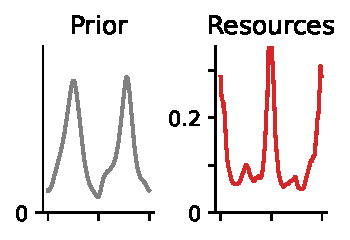
\includegraphics[width=0.15\textwidth]{figures/RunGardelle_FreePrior_CosineLoss_Downsampled_TargetSize_VIZ_EncPri.py_2_0-21_10.0_180_1000_4.pdf}
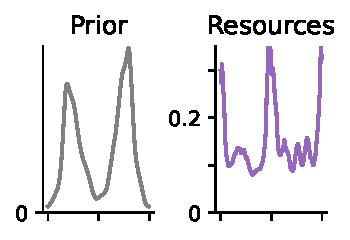
\includegraphics[width=0.15\textwidth]{figures/RunGardelle_FreePrior_CosineLoss_Downsampled_TargetSize_VIZ_EncPri.py_2_0-21_10.0_180_1000_5.pdf}
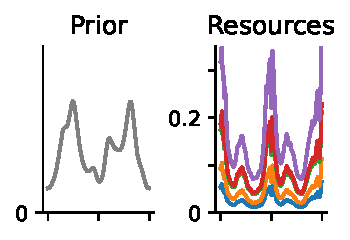
\includegraphics[width=0.15\textwidth]{figures/RunGardelle_FreePrior_CosineLoss_Downsampled_TargetSize_VIZ_EncPri.py_2_0-21_10.0_180_1000_1-2-3-4-5.pdf}

Fitting at $p=4$

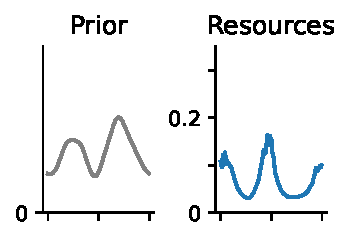
\includegraphics[width=0.15\textwidth]{figures/RunGardelle_FreePrior_CosineLoss_Downsampled_TargetSize_VIZ_EncPri.py_4_0-21_10.0_180_1000_1.pdf}
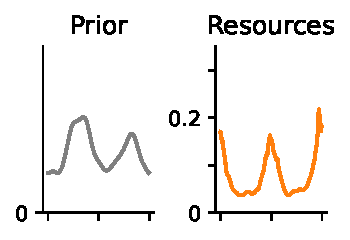
\includegraphics[width=0.15\textwidth]{figures/RunGardelle_FreePrior_CosineLoss_Downsampled_TargetSize_VIZ_EncPri.py_4_0-21_10.0_180_1000_2.pdf}
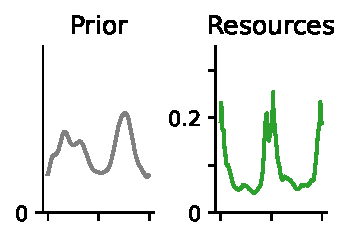
\includegraphics[width=0.15\textwidth]{figures/RunGardelle_FreePrior_CosineLoss_Downsampled_TargetSize_VIZ_EncPri.py_4_0-21_10.0_180_1000_3.pdf}
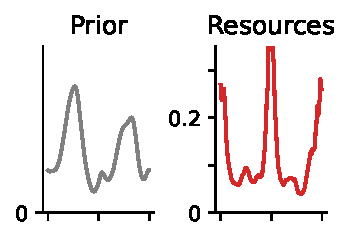
\includegraphics[width=0.15\textwidth]{figures/RunGardelle_FreePrior_CosineLoss_Downsampled_TargetSize_VIZ_EncPri.py_4_0-21_10.0_180_1000_4.pdf}
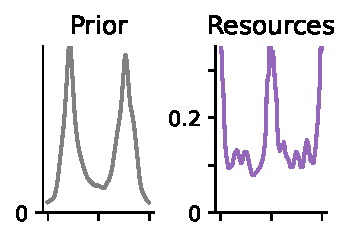
\includegraphics[width=0.15\textwidth]{figures/RunGardelle_FreePrior_CosineLoss_Downsampled_TargetSize_VIZ_EncPri.py_4_0-21_10.0_180_1000_5.pdf}
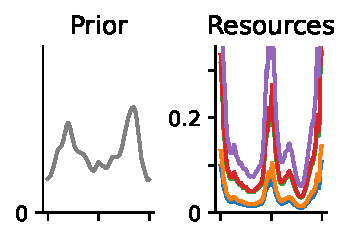
\includegraphics[width=0.15\textwidth]{figures/RunGardelle_FreePrior_CosineLoss_Downsampled_TargetSize_VIZ_EncPri.py_4_0-21_10.0_180_1000_1-2-3-4-5.pdf}

Fitting at $p=6$

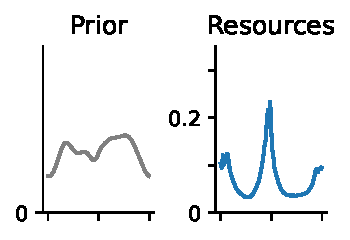
\includegraphics[width=0.15\textwidth]{figures/RunGardelle_FreePrior_CosineLoss_Downsampled_TargetSize_VIZ_EncPri.py_6_0-21_10.0_180_1000_1.pdf}
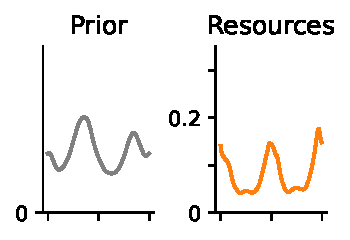
\includegraphics[width=0.15\textwidth]{figures/RunGardelle_FreePrior_CosineLoss_Downsampled_TargetSize_VIZ_EncPri.py_6_0-21_10.0_180_1000_2.pdf}
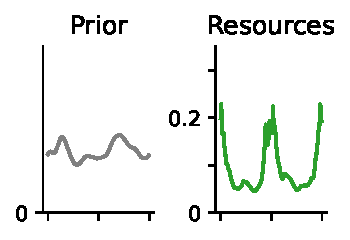
\includegraphics[width=0.15\textwidth]{figures/RunGardelle_FreePrior_CosineLoss_Downsampled_TargetSize_VIZ_EncPri.py_6_0-21_10.0_180_1000_3.pdf}
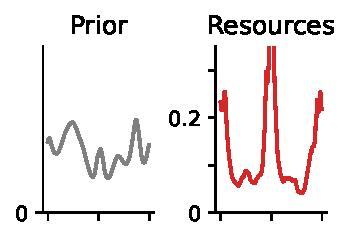
\includegraphics[width=0.15\textwidth]{figures/RunGardelle_FreePrior_CosineLoss_Downsampled_TargetSize_VIZ_EncPri.py_6_0-21_10.0_180_1000_4.pdf}
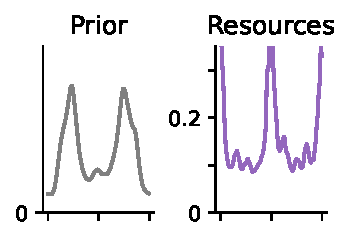
\includegraphics[width=0.15\textwidth]{figures/RunGardelle_FreePrior_CosineLoss_Downsampled_TargetSize_VIZ_EncPri.py_6_0-21_10.0_180_1000_5.pdf}
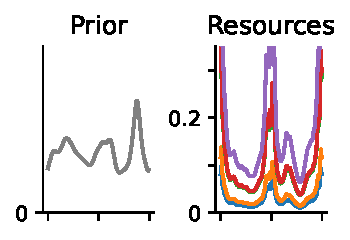
\includegraphics[width=0.15\textwidth]{figures/RunGardelle_FreePrior_CosineLoss_Downsampled_TargetSize_VIZ_EncPri.py_6_0-21_10.0_180_1000_1-2-3-4-5.pdf}

Fitting at $p=8$

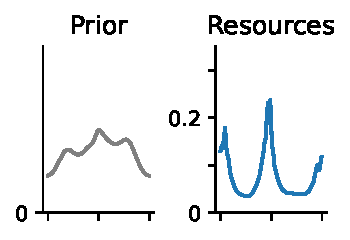
\includegraphics[width=0.15\textwidth]{figures/RunGardelle_FreePrior_CosineLoss_Downsampled_TargetSize_VIZ_EncPri.py_8_0-21_10.0_180_1000_1.pdf}
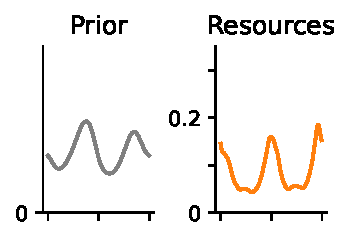
\includegraphics[width=0.15\textwidth]{figures/RunGardelle_FreePrior_CosineLoss_Downsampled_TargetSize_VIZ_EncPri.py_8_0-21_10.0_180_1000_2.pdf}
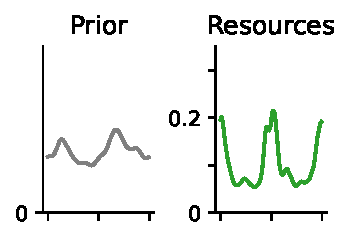
\includegraphics[width=0.15\textwidth]{figures/RunGardelle_FreePrior_CosineLoss_Downsampled_TargetSize_VIZ_EncPri.py_8_0-21_10.0_180_1000_3.pdf}
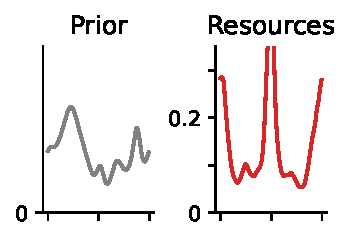
\includegraphics[width=0.15\textwidth]{figures/RunGardelle_FreePrior_CosineLoss_Downsampled_TargetSize_VIZ_EncPri.py_8_0-21_10.0_180_1000_4.pdf}
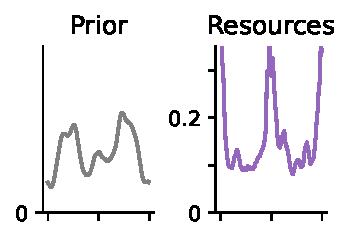
\includegraphics[width=0.15\textwidth]{figures/RunGardelle_FreePrior_CosineLoss_Downsampled_TargetSize_VIZ_EncPri.py_8_0-21_10.0_180_1000_5.pdf}
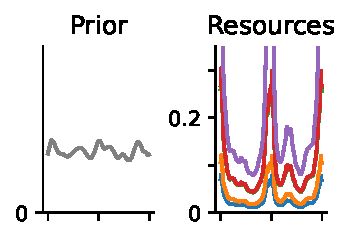
\includegraphics[width=0.15\textwidth]{figures/RunGardelle_FreePrior_CosineLoss_Downsampled_TargetSize_VIZ_EncPri.py_8_0-21_10.0_180_1000_1-2-3-4-5.pdf}


\caption{Orientation perception (data collected by \citep{deGardelle2010AnOI}). Fitting to 1K trials from the dataset of de Gardelle et al at one level of noise (left=large noise, right=small noise; first five column) or at all five levels (rightmost column). In each case, we show the prior (left) and the encoding (right). Coloring of noise levels is as in Main Paper, Figures 6--7. When fitting at a single level of noise, the encoding is fitted consistently even across loss functions, in accordance with the theory. However, the prior is fitted inconsistently: fitting with low exponents consistently leads to a prior peaking at oblique directions; fitting with higher exponents leads to a variety of results. As model fit is very similar across loss function exponents at one level of noise, for each level of sensory noise (Main Paper, Figure 7), loss function and prior are not identifiable. In contrast, when combining noise levels, model fit vary between loss functions (Main Paper, Figure 7). At high exponents, an approximately uniform prior is fitted.
Compare Main Paper, Figure 7 for the fit at $p=8$ on the full dataset (9,936 trials), which is highly consistent with the fit obtained at 1K trials but five noise levels.
}
\label{fig:gardelle-one-level-pri-enc}
\end{figure}

\begin{figure}
\centering
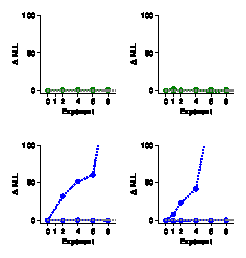
\includegraphics[width=0.5\textwidth]{figure8_Rec_FreeSI.pdf}
\caption{Model fit statistics for simulated datasets based on the data collected by \citet{Remington2018LateBI}, when presuming an encoding consistent with Weber's law (left, same as Main Paper, Figure 8i) or with a freely fitted encoding (right).
Coding of color and line type is as in Main Paper Figure 8i.
Even when the encoding is freely fitted, the bimodal prior (dotted, blue) allows identification of the loss function when data at multiple levels of noise is available.
}\label{fig:remington-nll-free-or-weber}
\end{figure}



\end{document}
